\documentclass[11pt,a4paper]{article}
\usepackage[T1]{fontenc}
\usepackage{lmodern}
\usepackage[margin=2.2cm]{geometry}
\usepackage{amsmath,amssymb}
\usepackage{graphicx}
\usepackage{booktabs}
\usepackage{tabularx}
\usepackage{ltablex}
\keepXColumns
\usepackage{placeins}
\usepackage{microtype}
\usepackage{enumitem}
\usepackage[font=small,labelfont=bf]{caption}
\usepackage[dvipsnames]{xcolor}
\usepackage[most]{tcolorbox}
\usepackage{url}
\def\UrlBreaks{\do\/\do\_\do\.\do\-}
\usepackage[colorlinks=true,linkcolor=MidnightBlue,urlcolor=MidnightBlue]{hyperref}

\graphicspath{{../../analysis/cubic_stress_test/}{../../zero_thickness_plate/a3_re500_ell/}%
{../../zero_thickness_plate/figs/}{../../analysis/drag_even_fit/}{../../analysis/residue_test/}%
{../../analysis/fold_check/}}
\setlist{itemsep=2pt,topsep=4pt}
\newcommand{\CL}{C_L}
\newcommand{\CD}{C_D}
\newcommand{\CN}{C_N}
\newcommand{\CA}{C_A}
\newcommand{\supp}{\textcolor{ForestGreen}{\textbf{supported}}}
\newcommand{\rej}{\textcolor{BrickRed}{\textbf{rejected}}}
\newcommand{\wdn}{\textcolor{BrickRed}{\textbf{withdrawn}}}
\newcommand{\opn}{\textcolor{Goldenrod!80!black}{\textbf{open}}}
\newcommand{\weak}{\textcolor{Orange}{\textbf{weakened}}}
\newtcolorbox{keybox}[1]{breakable,colback=MidnightBlue!5,colframe=MidnightBlue,boxrule=0.8pt,arc=2pt,
  left=6pt,right=6pt,top=4pt,bottom=4pt,title={\bfseries #1},coltitle=white,colbacktitle=MidnightBlue}
\newtcolorbox{warnbox}[1]{breakable,colback=Goldenrod!12,colframe=BrickRed,boxrule=0.8pt,arc=2pt,
  left=6pt,right=6pt,top=4pt,bottom=4pt,title={\bfseries #1},coltitle=white,colbacktitle=BrickRed}

\title{The steady small-angle loads for the viscous Wagner problem\\[2pt]
\large Lift and drag of four bodies at ultra-low Reynolds number: findings, hypotheses, tests,
and what remains}
\author{Status report}
\date{Revision 3, 20 October 2026 (first issued 19 October 2026)}

\begin{document}
\maketitle

% =====================================================================================
\section*{Summary}

A step response is measured against the steady state it settles to, so the first task of the
programme is the steady load curve at small angles. Steady (SIMPLE) 2D laminar solutions were
computed for NACA0012, NACA0006, a $2.3\%$-thick stadium plate and a zero-thickness plate, with the angle
set by rotating the freestream on one mesh per body and Reynolds number. Lift is odd in $\alpha$ and
drag is even:
\[
\CL = a_1\theta + a_3\theta^3 + a_5\theta^5 + \dots,\qquad
\CD = d_0 + d_2\theta^2 + d_4\theta^4 + \dots
\]
Both are fitted with Legendre polynomials on windows $0$--$A$ and converted to powers of $\theta$.

\begin{keybox}{Findings (current state)}
\begin{enumerate}[leftmargin=*]
\item \textbf{The lift is analytic at the origin, with a finite, nonzero cubic term, for all four
  bodies.} The deficit $a_1\theta - \CL$ goes as $\theta^3$, with local exponent $3.01$--$3.10$ over
  $1$--$4^\circ$. There is no non-analytic term.
\item \textbf{$a_3$ is robust:} to $0.1\%$ against window and fit order, and against re-converged data at Re
  500 and 700. At Re 900 it moves by $0.5\%$, still inside the $\approx1\%$ mesh uncertainty. At Re 500:
  $a_3 = -28.2$, $-24.9$, $-18.9$, $-12.8$ from NACA0012 to the zero-thickness plate.
\item \textbf{The production solver tolerances biased the higher coefficients} (Section~\ref{sec:tight}).
  The production runs stall $10^{-7}$--$2\times10^{-5}$ in $\CL$ short of the fixed point, by an error smooth
  in $\alpha$ that the fits absorb invisibly. Re-converged (``tight'') data for the zero-thickness plate
  give $a_5 = -367\pm2$, $-376\pm4$, $-313\pm2$ at Re 500, 700, 900. The production values were off by
  $3\%$ to over $50\%$, and $|a_5|$ does not grow with Re.
\item \textbf{The two-term radius estimates agree at each Re:} about $10.7^\circ$, $9.5^\circ$ and $9.4^\circ$.
  Padé and AAA fits put a real-axis pole at $10.7$--$11.0^\circ$ (Re 500), with a zero just before it
  (Section~\ref{sec:pade}).
\item \textbf{Drag is a far cleaner signal than lift} (Section~\ref{sec:drag}): fit residuals of
  $2$--$7\times10^{-10}$. $d_0$, $d_2$ and $d_4$ are resolved at Re 500--900 and all positive. The net
  leading-edge-suction fraction $\eta$ rises with Re ($0.74\to0.79$) and with thinness ($0.66\to0.74$
  at Re 500).
\item \textbf{$\CD$ shows no consistent singularity; $\CL$, $\CN$ and $\CA$ do.} A shared-denominator
  residue test (Section~\ref{sec:residue}) puts the singular part of the force within about $0.3^\circ$ of
  the lift axis, with $\CD$'s singular amplitude about $0.5\%$ of $\CL$'s. This rests on the calibrated
  routes only; neither stated verdict rule confirms it.
\item \textbf{The first fold-test results argue against a real-axis fold below $9^\circ$}
  (Section~\ref{sec:fold}). The steady branch at Re 500 continues smoothly to $9^\circ$, with $\CL$'s slope
  falling, not steepening, toward a maximum near $9$--$9.5^\circ$. The polynomial fits extrapolate to
  $6$--$9^\circ$ 4--10 times better than the Padé and square-root models. The square-root model's branch
  point at $8.92^\circ$ is contradicted on this branch. Runs at $9.5$--$12^\circ$, ascending and
  descending, are in progress.
\end{enumerate}
\end{keybox}

\begin{warnbox}{Claims from earlier revisions that are corrected or withdrawn}
\begin{itemize}[leftmargin=*]
\item \emph{``$\CL$ is repeatable to $10^{-8}$, so the coefficients are noise-limited.''} The $10^{-8}$ was
  the repeatability of a stalled state. The production $a_5$, $a_7$ and radius values are superseded by
  the re-converged ones (Section~\ref{sec:tight}).
\item \emph{``For the zero-thickness plate the radius shrinks as $\mathrm{Re}^{-0.63}$ and $|a_5|$ grows
  3--5$\times$ from Re 200 to 900.''} Withdrawn for Re 500--900; Re 200--400, 600 and 800 are not yet
  re-converged.
\item \emph{``$a_3$ is fixed to $0.1\%$ for every body.''} Correct only up to Re 700 for the zero-thickness
  plate; $0.5\%$ at Re 900.
\item \emph{``The zero-thickness plate's deficit grows as $\theta^{3.4}$.''} An H-grid mesh artefact
  (Section~\ref{sec:mesh}).
\item \emph{``A square-root branch point at $8.92^\circ$''} (from fitting the tight data) is contradicted
  by a smooth steady solution at $9^\circ$ (Section~\ref{sec:fold}).
\item \emph{``The thick plate's non-monotonic $a_3(\mathrm{Re})$ comes from its sharp leading edge.''} Its
  premise is wrong: the plate's leading-edge radius ($0.0115c$) is larger than NACA0006's ($0.0040c$).
  The wording is listed in \texttt{SHARP\_LE\_CORRECTIONS.md} for revision.
\end{itemize}
\end{warnbox}

\newpage
% =====================================================================================
\section{Setup}

\begin{itemize}[leftmargin=*]
\item \textbf{Solver.} OpenFOAM (Foundation) \texttt{foamRun}, incompressible, steady SIMPLE, with the same
  schemes as the transient campaign.
\item \textbf{Two tolerance levels} (Section~\ref{sec:tight}):
  \begin{itemize}
  \item \emph{production}: p \texttt{tolerance 1e-7}, U \texttt{1e-8}, \texttt{relTol 0.01},
    6000--12000 iterations;
  \item \emph{tight}: tolerance $10^{-12}$, same relTol, continued for $\ge3000$ iterations.
  \end{itemize}
  Convergence is judged on the force trace, never on the residuals. A tight case counts when its last
  $500$ iterations move the coefficient by $\le3\times10^{-9}$ and the geometrically extrapolated
  remainder is also $\le3\times10^{-9}$.
\item \textbf{Bodies and meshes.} One mesh per body and Re; the first cell is
  $h_1 = 0.05/\sqrt{\mathrm{Re}}$.
  \begin{itemize}
  \item \emph{NACA0012, NACA0006:} an O-ring, cut at $0.98c$ (blunt trailing edge).
  \item \emph{Plate, $t/c=0.023$:} a stadium section, semicircular edges of radius $0.0115c$.
  \item \emph{Zero-thickness plate:} confocal elliptic coordinates $z = c/2 + (c/2)\cosh(\mu + i\nu)$, the
    plate at $\mu=0$, with $n_\nu = 800\sqrt{\mathrm{Re}/500}$ (E800 at Re 500). The plate is an internal
    surface, split into two walls by \texttt{createBaffles}.
  \end{itemize}
\item \textbf{Angles.} $0$--$6^\circ$ every $0.25^\circ$ at Re 500, and every $0.5^\circ$ in the Re sweeps
  (Re 200--900). The tight re-convergence covers $0.25$--$5^\circ$ at $0.25^\circ$ for Re 500, 700 and 900.
  The fold test adds $7$--$12^\circ$ at Re 500.
\item \textbf{OpenFOAM builds.}
  \begin{itemize}
  \item dev, 13 and v14 agree to about $4\times10^{-7}$ in $\CL$.
  \item Two v14 snapshots were in use: package 20260724 (\path{14-7b05503f98a8}) and package 20261008
    (\path{14-a4867fc914c1}). Their difference is unmeasured, so each Re's tight runs were kept on one
    build. The same build on different hardware and rank counts agrees to $6\times10^{-12}$.
  \end{itemize}
\end{itemize}

% =====================================================================================
\section{Is the lift cubic at the origin? The deficit test}

For $\CL = a_1\theta + a_3\theta^3 + \dots$ the deficit $d = a_1\theta - \CL \to -a_3\theta^3$, so
$d/\theta^3$ tends to a constant and the local exponent $\mathrm{d}\ln d/\mathrm{d}\ln\theta$ tends to $3$.
Here $a_1$ is the Richardson limit of $\CL/\theta$ from $0.25^\circ$ and $0.5^\circ$. A non-analytic term
such as $\theta^{3+\epsilon}$ or $\theta^3\ln\theta$ would fail this test.

\begin{figure}[htbp]\centering
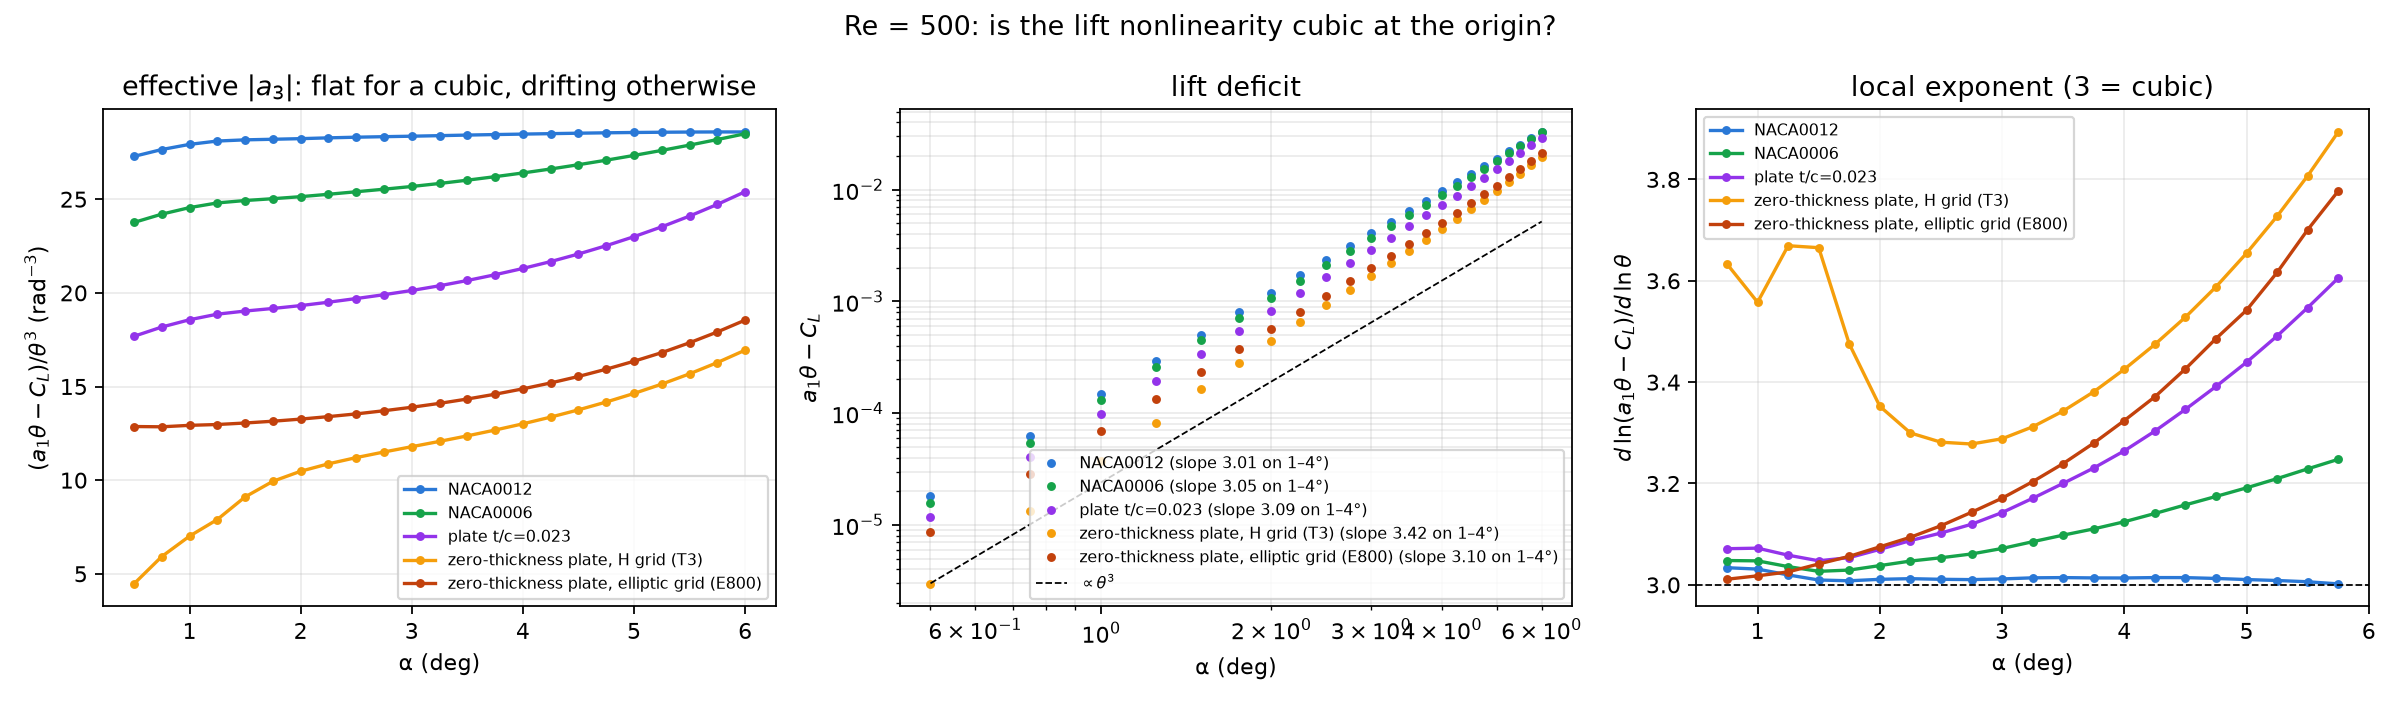
\includegraphics[width=\linewidth]{deficit_four_bodies.png}
\caption{Re $=500$, production data. Left: $d/\theta^3$. Centre: the deficit, log--log. Right: its
local exponent. Yellow is the superseded H-type grid of the zero-thickness plate.}
\end{figure}

\begin{center}\small
\begin{tabular}{lrrrrrrr}
\toprule
body & $a_1$ & exponent, $1$--$4^\circ$ & \multicolumn{5}{c}{$d/\theta^3$ at $0.5,\ 1,\ 2,\ 4,\ 6^\circ$}\\
\midrule
NACA0012 & 3.271 & 3.01 & 27.3 & 27.9 & 28.2 & 28.5 & 28.6\\
NACA0006 & 4.240 & 3.05 & 23.8 & 24.6 & 25.1 & 26.4 & 28.5\\
plate $t/c=0.023$ & 4.825 & 3.09 & 17.7 & 18.6 & 19.3 & 21.3 & 25.4\\
zero-thickness plate & 4.935 & 3.10 & 12.9 & 12.9 & 13.3 & 14.9 & 18.5\\
\midrule
\textcolor{gray}{zero-thickness, H-grid} & \textcolor{gray}{4.908} & \textcolor{gray}{3.42} &
\textcolor{gray}{4.5} & \textcolor{gray}{7.0} & \textcolor{gray}{10.5} & \textcolor{gray}{13.0} & \textcolor{gray}{16.9}\\
\bottomrule
\end{tabular}
\end{center}

All four bodies pass. The production bias of Section~\ref{sec:tight} is $\le2\times10^{-5}$, which is
negligible against deficits of $10^{-4}$--$10^{-2}$, so this test stands.

% =====================================================================================
\section{The zero-thickness plate: mesh}\label{sec:mesh}

\begin{figure}[htbp]\centering
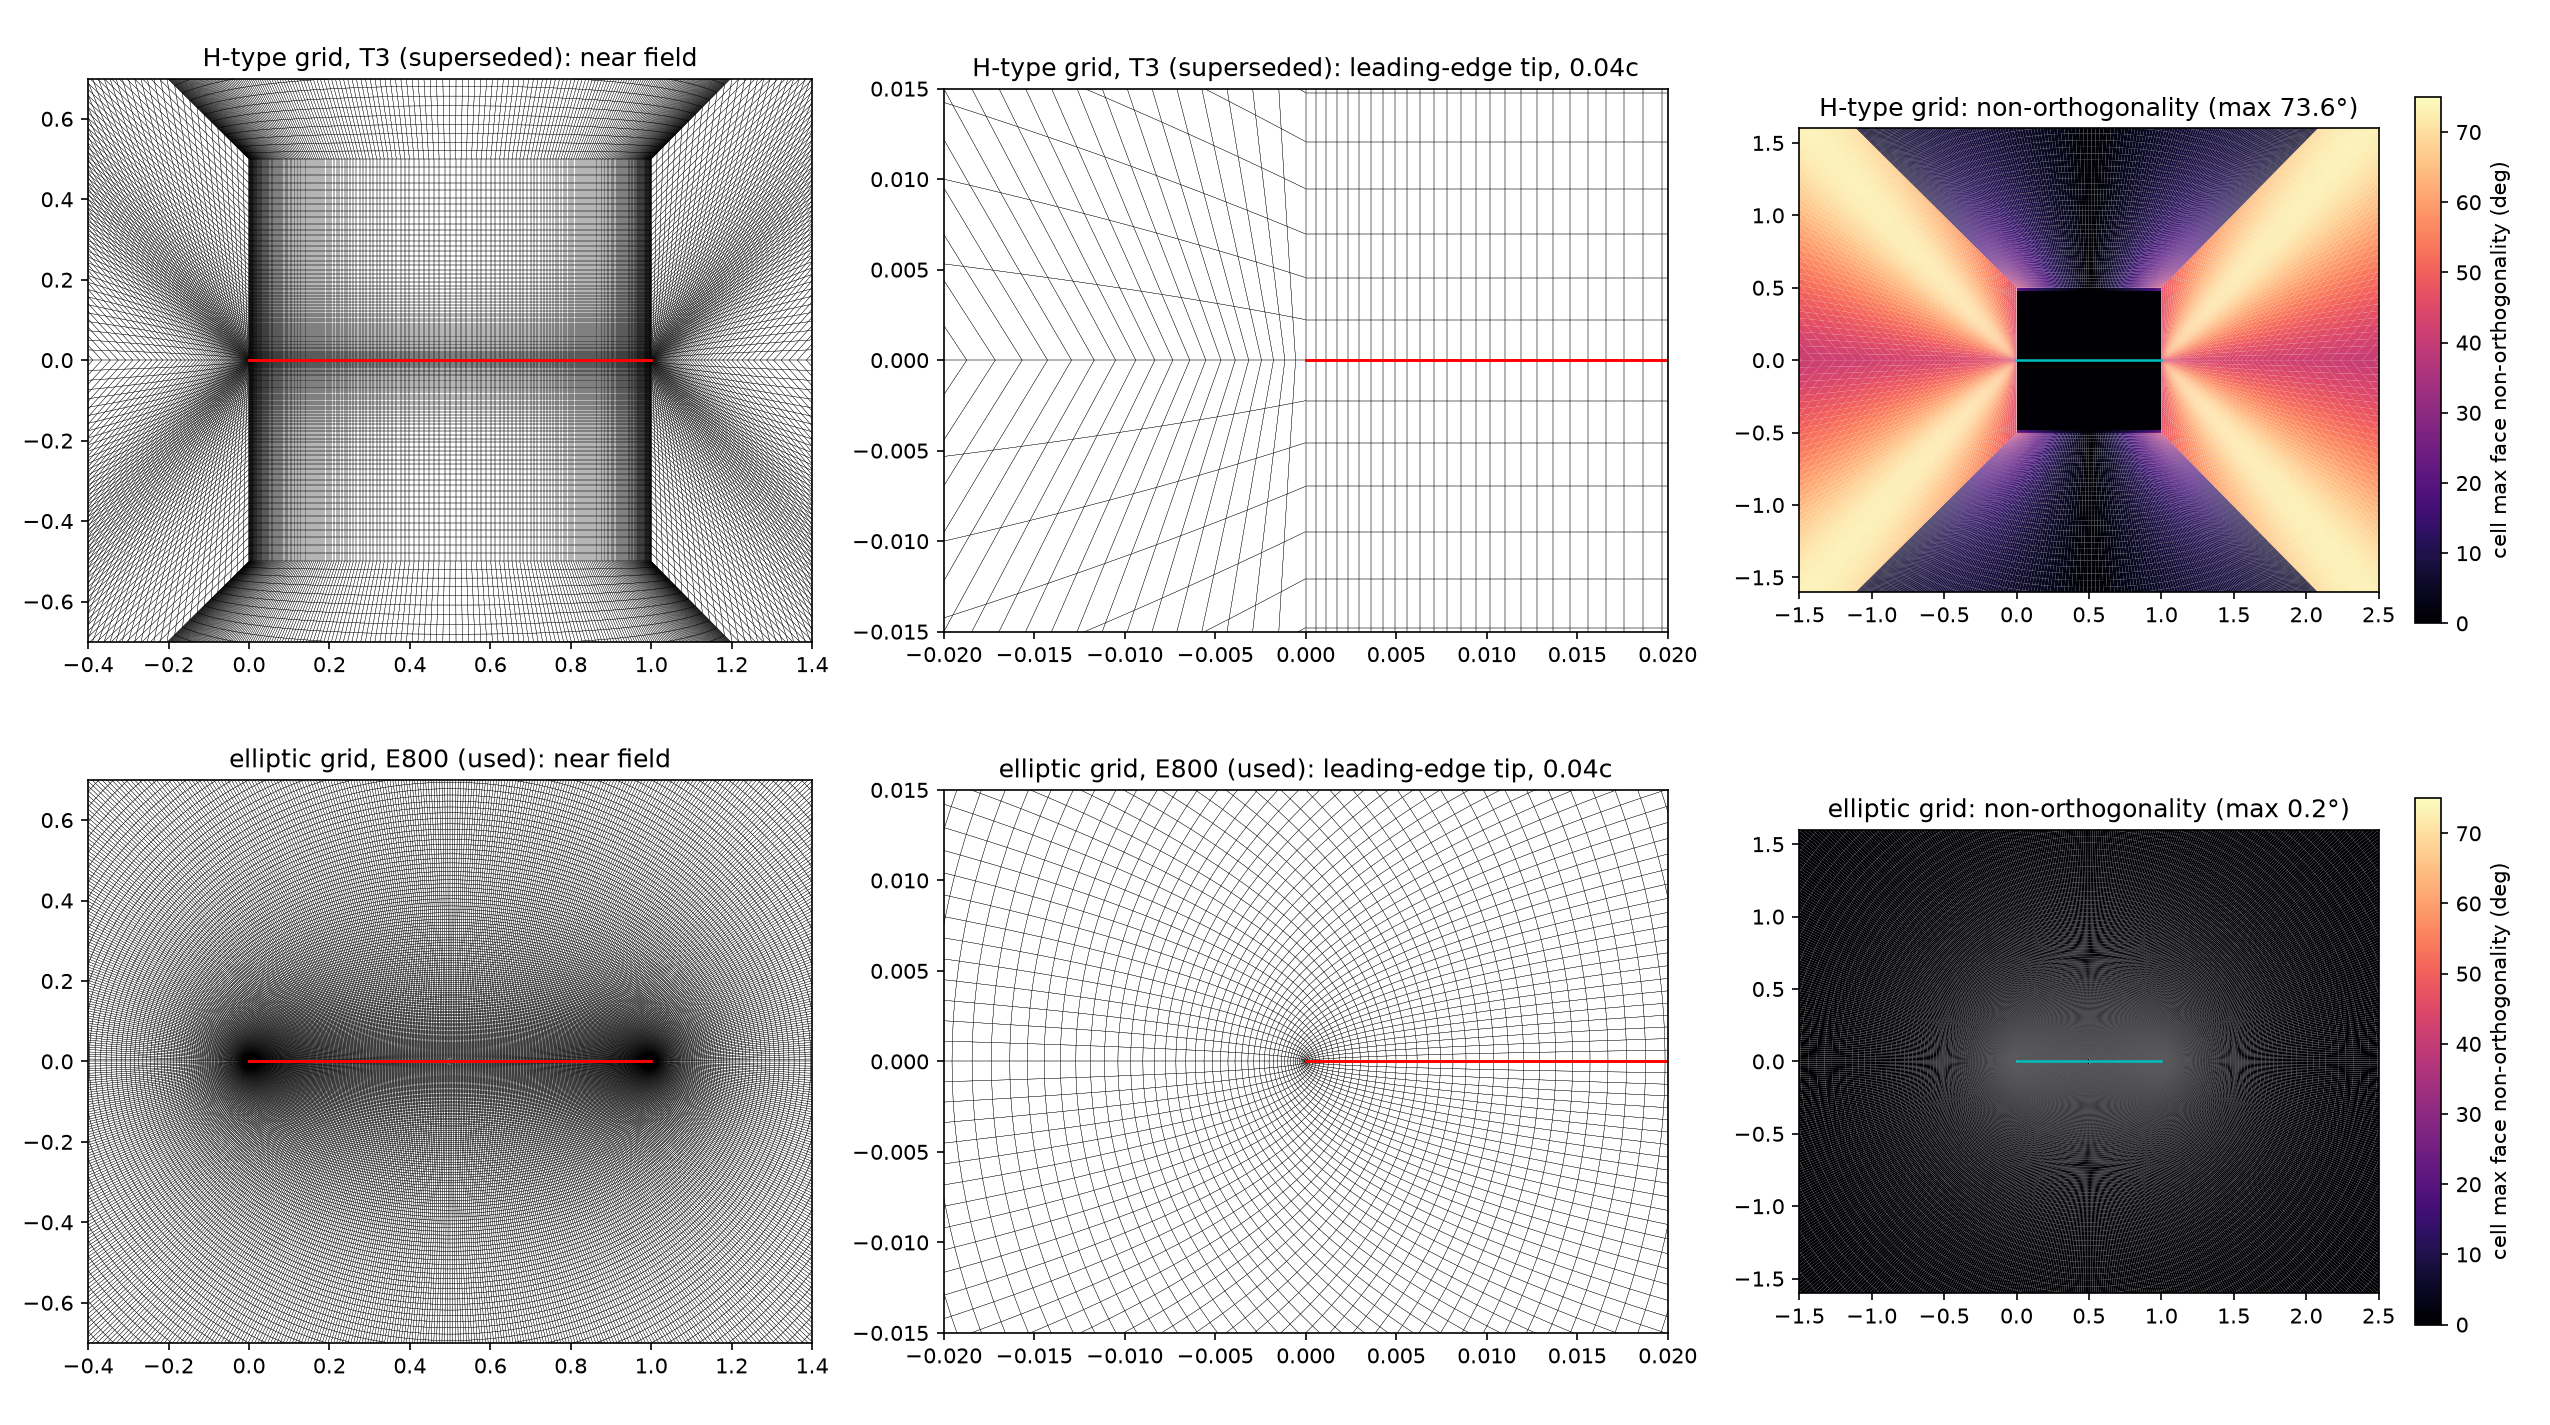
\includegraphics[width=\linewidth]{mesh_comparison.png}
\caption{Top: the H-type grid (T3), the topology of the user's original \texttt{.geo}. Bottom: the
elliptic grid (E800). Columns: near field; the $0.04c$ around the leading-edge tip; non-orthogonality.}
\end{figure}

\begin{itemize}[leftmargin=*]
\item \textbf{H-type grid.} Its wedges reach $73.6^\circ$ (T3) to $76.2^\circ$ (T4) non-orthogonality,
  $54^\circ$ within $0.02c$ of a tip. Tip refinement at $6^\circ$ did not converge monotonically. This grid
  produced the spurious $\theta^{3.4}$.
\item \textbf{Elliptic grid.} Orthogonal by construction (maximum $4.5^\circ$, mostly from the span
  direction), and clustered at the tips by itself: tip cell $1.5\times10^{-5}c$ at Re 500.
\item \textbf{Mesh sensitivity} (E560 against E800, production): $\Delta\CL = +0.0026\,\theta - 0.083\,\theta^3$,
  mostly a slope change. $a_3$ moves by $0.65\%$; the extrapolated $a_3 \approx -12.8$ to $-13.0$. The mesh
  sensitivity of $a_5$ and of the drag coefficients has not been measured.
\end{itemize}

% =====================================================================================
\section{Robustness of $a_3$, and what $a_5$ adds (production data, four bodies)}

\begin{figure}[htbp]\centering
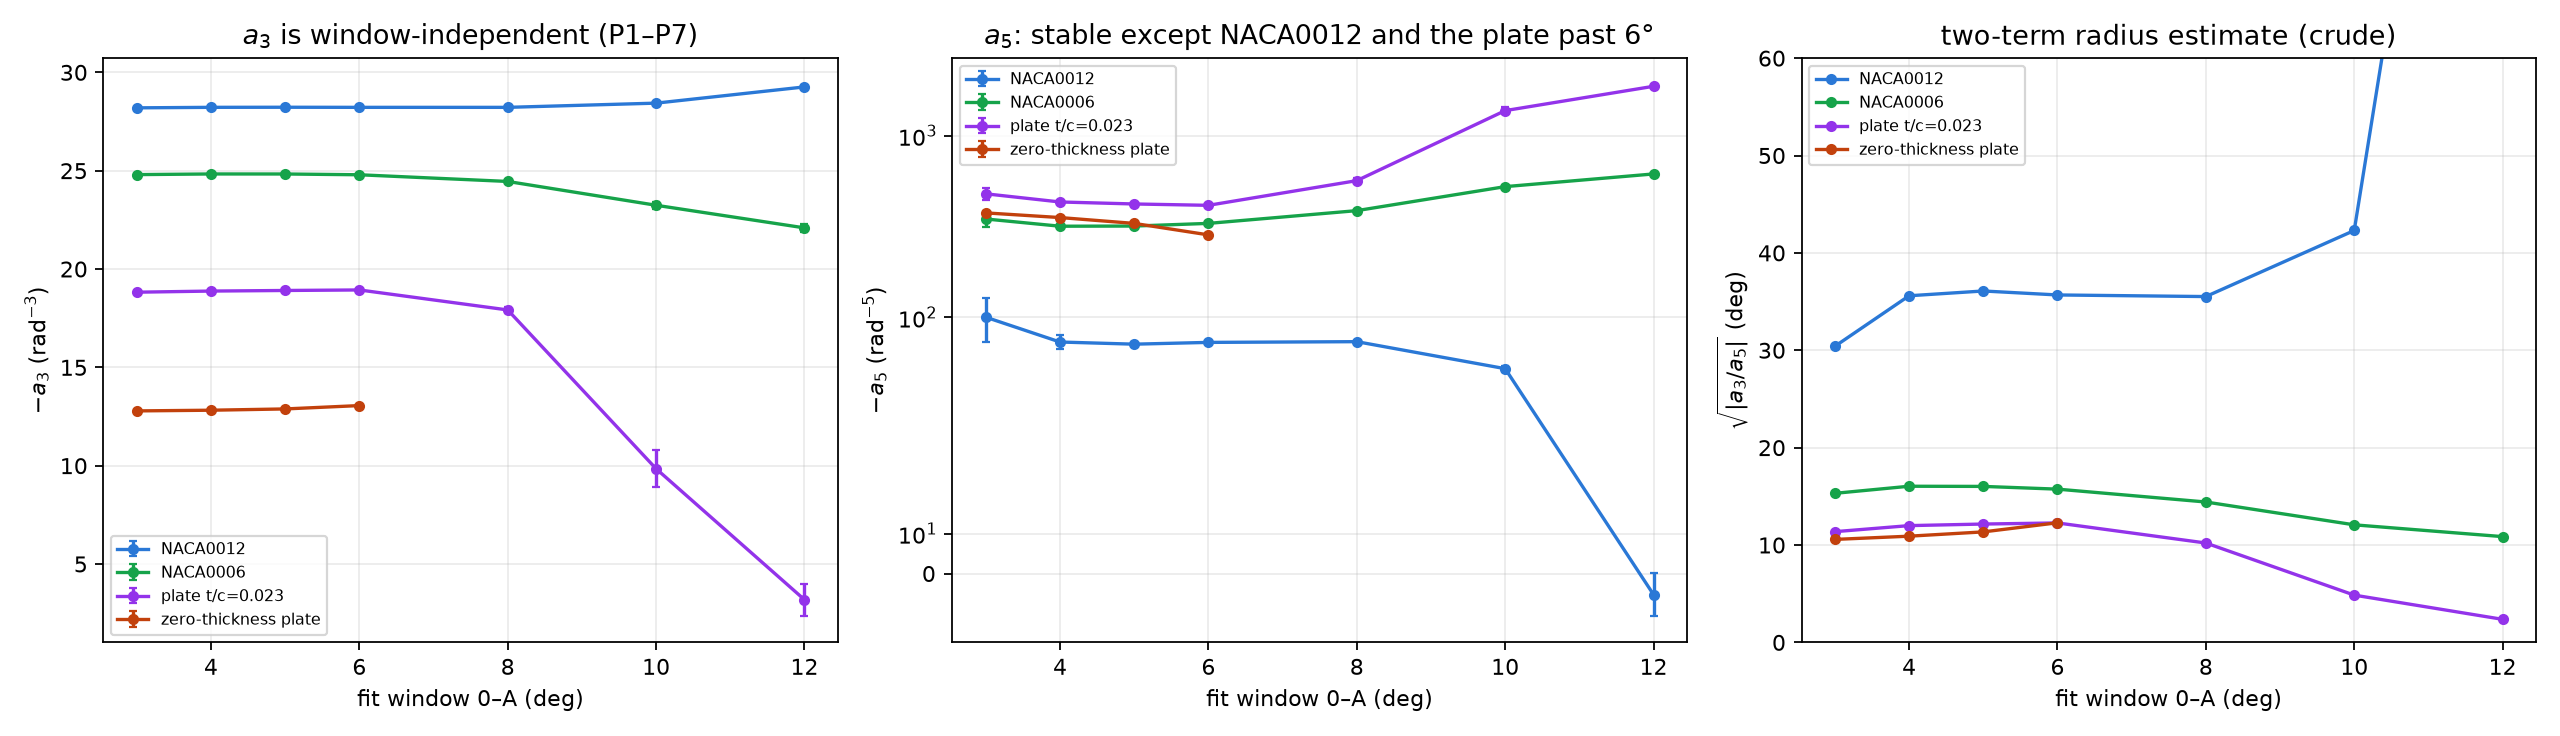
\includegraphics[width=\linewidth]{coefficients_vs_window.png}
\caption{Re $=500$, production data, P1--P7 fits on $0$--$A$ with least-squares error bars: $a_3$ (left),
$a_5$ (centre), and $\sqrt{|a_3/a_5|}$ (right).}
\end{figure}

\begin{itemize}[leftmargin=*]
\item \textbf{$a_3$ is window- and order-independent within each body's validity range}, to $0.1\%$:
  $-28.22\pm0.01$ (NACA0012, $3$--$8^\circ$), $-24.8$ (NACA0006), $-18.9$ (plate), $-12.79$ (zero-thickness
  plate, production; tight $-12.806$).
\item \textbf{$a_5$ has the sign of $a_3$ for all four bodies:} $-72$, about $-310$, $-420$ and $-380$
  (production; tight $-367$ for the zero-thickness plate). The three bodies without tight runs carry the
  same bias risk.
\item \textbf{Beyond the validity range every coefficient becomes window-dependent:} from about
  $10^\circ$ for NACA0012, and $8^\circ$ for NACA0006 and the plate. For the plate that is its leading-edge
  bubble range: formation at $7.9^\circ$, and reattachment reaching the trailing edge at $8.4^\circ$, at Re
  500.
\end{itemize}

\begin{figure}[htbp]\centering
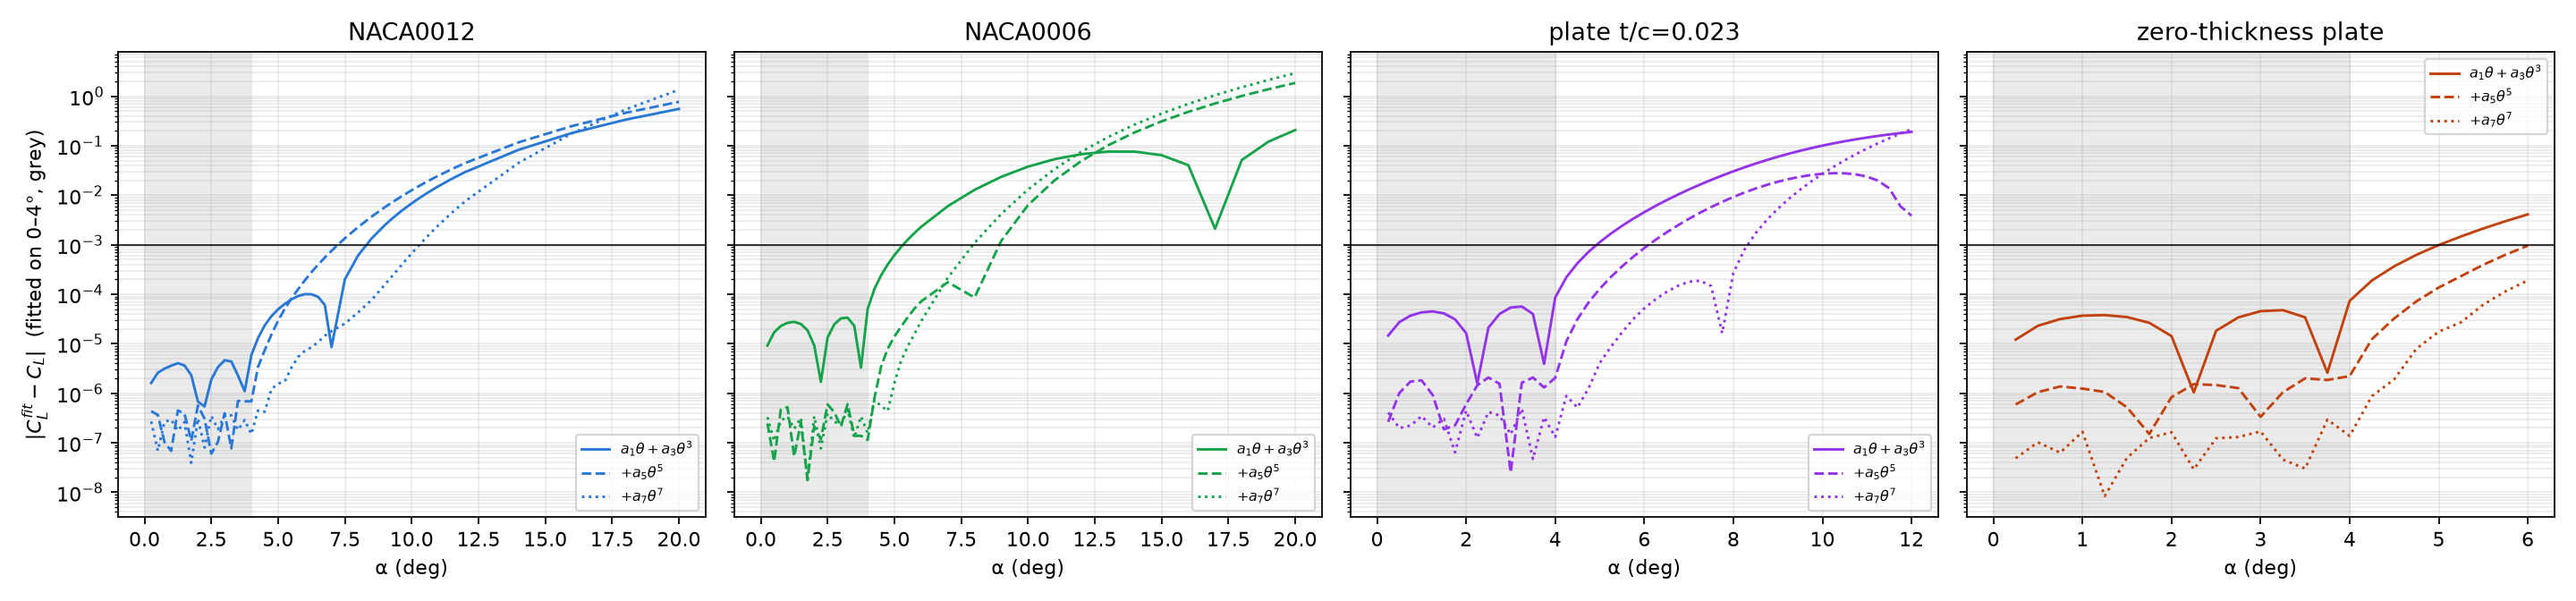
\includegraphics[width=\linewidth]{extrapolation.png}
\caption{Truncations fitted on $0$--$4^\circ$ (grey band), extrapolated. Horizontal line: $10^{-3}$.}
\end{figure}

\begin{center}\small
\begin{tabular}{lccc}
\toprule
first miss $>10^{-3}$ & $a_1\theta+a_3\theta^3$ & $+a_5\theta^5$ & $+a_7\theta^7$\\
\midrule
NACA0012 & $8.5^\circ$ & $7.5^\circ$ & $10.5^\circ$\\
NACA0006 & $5.5^\circ$ & $9^\circ$ & $8^\circ$\\
plate $t/c=0.023$ & $5^\circ$ & $6.25^\circ$ & $8.5^\circ$\\
zero-thickness plate & $5.25^\circ$ & $>6^\circ$ (end of data) & $>6^\circ$ (end of data)\\
\bottomrule
\end{tabular}
\end{center}

% =====================================================================================
\section{The solver-tolerance bias, and the re-converged coefficients}\label{sec:tight}

\textbf{The mechanism.} A linear solve stops at whichever comes first, $r <$ tolerance or $r <$
relTol$\cdot r_0$. With p tolerance $10^{-7}$ and relTol $0.01$, relTol binds only while
$r_0 > 10^{-5}$. Late in a run the absolute tolerance binds instead. U solves then do $0$ iterations and p
solves $0$--$2$, so each SIMPLE iteration removes almost nothing. SIMPLE contracts the error by only
$\rho\approx0.998$ per iteration, so the run stalls about step$/(1-\rho)$ from the fixed point:
$10^{-7}$--$2\times10^{-5}$ in $\CL$, growing with $\alpha$. The tight settings (tolerance $10^{-12}$) keep
relTol binding throughout.

\textbf{Why the window test missed it.}
\begin{itemize}[leftmargin=*]
\item With every angle run the same way, the error is smooth in $\alpha$. Every fit window shifts together,
  and the spread/standard-error test passes. Re 700's production $a_5$ ($-405\pm1$, $-409\pm1$) was stable
  and $8\%$ wrong.
\item With angles run two ways (the separately seeded $0.25^\circ$ quarter angles against the $0.5^\circ$
  grid), neighbours stall on opposite sides, and the mixed data fit as noise (rms $4\times10^{-7}$).
\item No test confined to one data set can detect a bias common to all of it; only converged data can.
\end{itemize}

\begin{center}\small
\resizebox{\linewidth}{!}{%
\begin{tabular}{rlcccccc}
\toprule
\multicolumn{8}{c}{zero-thickness plate, re-converged (production values in brackets)}\\
Re & angles used & $a_1$ & $a_3$ & $a_5$ & $a_7$ & $\sqrt{|a_3/a_5|}$ & $\sqrt{|a_5/a_7|}$\\
\midrule
500 & $0.25$--$4.25^\circ$ (17) & 4.93491 & $-12.806$ ($-12.79$) & $-367\pm2$ ($-380$) & $\approx-9500\pm1000$ & $10.7^\circ$ & $10$--$11^\circ$\\
700 & $0.25$--$3.75^\circ$ (15) & 5.06595 & $-10.528$ ($-10.52$) & $-376\pm4$ ($-405$ to $-482$) & $\approx-1.2$ to $-1.6\times10^4$ & $9.5^\circ$ & $8.6$--$10.4^\circ$\\
900 & $0.25$--$4^\circ$ (12) & 5.15642 & $-8.342$ ($-8.30$) & $-313\pm2$ ($-485$ to $-805$) & $\approx-1.1$ to $-1.25\times10^4$ & $9.4^\circ$ & $9.0$--$9.6^\circ$\\
\bottomrule
\end{tabular}}
\end{center}

\begin{itemize}[leftmargin=*]
\item $a_5$ is resolved at all three Re: the window spread is $1$--$3$ standard errors. At Re 900 this
  needs P1--P11 on $0$--$4^\circ$; P1--P9 leaves a $10^{-8}$ residual. $a_7$ is borderline
  ($\pm10$--$20\%$, sensitive to the fit order); $a_9$ and $a_{11}$ are not resolved.
\item $a_3$ still falls almost linearly with Re: by $1.14$ per $100$ over Re 500--700, and $1.09$ over
  700--900.
\item At Re 900, every resolved coefficient from $a_3$ to $a_{11}$ is negative.
\end{itemize}

% =====================================================================================
\section{Locating the singularity: Padé and AAA (Re 500)}\label{sec:pade}

$\CL = \theta\,g(z)$ with $z=\theta^2$. A pole of a rational approximant of $g$ at $z_p$ means a singularity at
$\theta=\pm\sqrt{z_p}$: on the real axis if $z_p>0$, on the imaginary axis if $z_p<0$, a complex pair
otherwise.

\textbf{Three routes:}
\begin{itemize}[leftmargin=*]
\item \textbf{A: classical Padé of the fitted Taylor coefficients} (\texttt{scipy.interpolate.pade}).
  It fails: the poles jump between $4^\circ$ and $26^\circ$, because a Padé of a series amplifies the
  $20$--$100\%$ uncertainty in $a_9$ and $a_{11}$.
\item \textbf{B: rational least squares} $\CL = \theta P_L(z)/Q_M(z)$, fitted to the data, with
  Sanathanan--Koerner reweighting and $z$ scaled to $[0,1]$.
\item \textbf{C: AAA} (\texttt{scipy.interpolate.AAA}): barycentric form with its own doublet handling,
  independent of B's basis.
\end{itemize}

\textbf{Froissart doublets.} A pole with a zero almost on top of it is a noise-fitting artefact. A pole
counts as genuine only if it has no zero within $1\%$ (in $z$), a non-negligible residue, and stability
across orders, windows and noise. In the [3/2] fit, the pole at $3.11^\circ$ has a zero on top of it, a
residue of $1.2\times10^{-8}$ and a contribution of $2\times10^{-9}$ to $\CL$; it moves between $2.5$ and
$6.3^\circ$ with the order. The pole at $10.85^\circ$ has its nearest zero $9\%$ away, a residue of $3.1$ and a
contribution of $4\times10^{-2}$, and stays at $10.71$--$10.85^\circ$.

\begin{center}\small
\begin{tabular}{llcc}
\toprule
route & data & genuine nearest pole & zero before it\\
\midrule
B & tight, windows $0$--$3.5^\circ$ to $0$--$4.25^\circ$, orders [1/1]--[4/3] & $10.71$--$11.00^\circ$ & $10.26$--$10.37^\circ$\\
B & production, windows to $0$--$6^\circ$ & $10.71$--$11.31^\circ$ & $10.25$--$10.71^\circ$\\
C & tight, loose tolerance (2--4 terms) & $10.74$--$10.76^\circ$ & $10.28$--$10.30^\circ$\\
C & production, same angles & $10.68$--$10.79^\circ$ & $10.24$--$10.31^\circ$\\
\bottomrule
\end{tabular}
\end{center}

\begin{itemize}[leftmargin=*]
\item No complex or imaginary-axis pole appears nearer, in any route. Extra degrees of freedom only add
  doublets: the data resolve a single singular feature.
\item \textbf{Zero before pole} is how a Padé approximant represents a branch point with a positive
  exponent. The [1/1] Padé of $\sqrt{1-x}$ has its zero at $4/3$ and its pole at $4$, both beyond the true
  branch point at $1$. This pointed to a square-root singularity, such as a fold, at or below about
  $10.3^\circ$.
\item \textbf{Limits.} The [1/1] and [2/1] poles are the ratio estimates $\sqrt{|a_3/a_5|}$ and
  $\sqrt{|a_5/a_7|}$. The rational fits do not extrapolate better than the polynomial (now tested
  directly, Section~\ref{sec:fold}). And $10.8^\circ$ is 2.5 times beyond the data.
\end{itemize}

% =====================================================================================
\section{Drag: the even half of the expansion}\label{sec:drag}

Body axes split the force into a normal part $\CN = \CL\cos\theta + \CD\sin\theta$ (odd) and an axial
part $\CA = \CD\cos\theta - \CL\sin\theta$ (even). To second order these are tied exactly:
$n_1 = a_1 + d_0$ and $d_2 = n_1 + A_2 - A_0/2$. Both identities close, to $10^{-9}$ and $10^{-5}$. The
\textbf{net suction fraction} $\eta = -A_2/n_1$ equals $1$ for the potential flat plate
($\CA=-2\pi\theta^2$, $\CN=2\pi\theta$, no drag rise). In viscous flow $A_2$ also contains the change of
skin friction with $\alpha$, so $\eta$ is net of it.

\begin{figure}[htbp]\centering
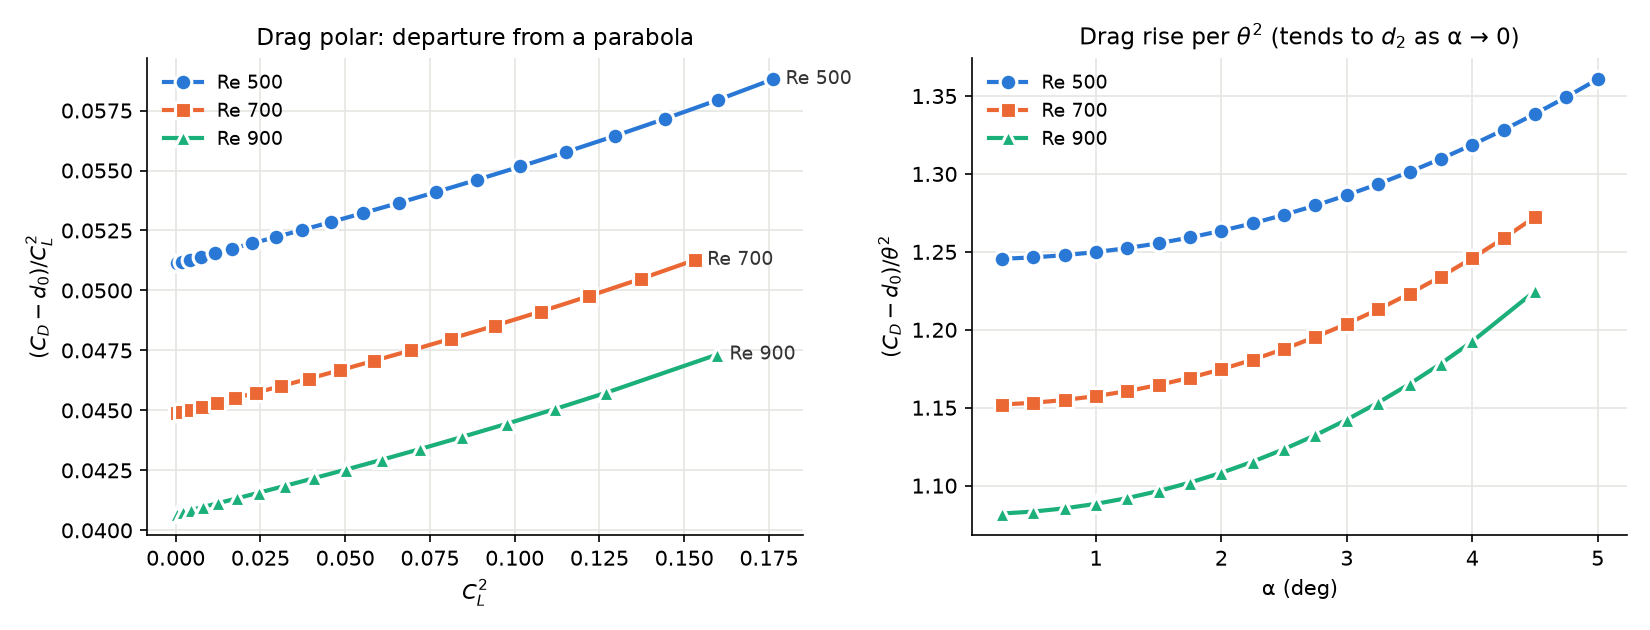
\includegraphics[width=\linewidth]{drag.png}
\caption{Zero-thickness plate, tight data. Left: $(\CD-d_0)/\CL^2$ against $\CL^2$, which is constant for
a parabolic polar. Right: $(\CD-d_0)/\theta^2$, which tends to $d_2$ as $\alpha\to0$.}
\end{figure}

\begin{itemize}[leftmargin=*]
\item \textbf{$\CD$ converges far better than $\CL$.} The tight tails move $10^{-11}$--$5\times10^{-10}$ per
  $500$ iterations, every tight angle is usable (including $4.5$--$5^\circ$, where $\CL$ is not), and the
  even fits leave rms $2$--$7\times10^{-10}$.
\item \textbf{Production $\CD$} is biased by $10^{-9}$--$8\times10^{-8}$ below $4.25^\circ$. Fitted, it gives
  $d_0$ and $d_2$ to $3\times10^{-5}$ and $d_4$ to $0.3$--$0.6\%$, but not $d_6$.
\item \textbf{The $\alpha=0$ point} must pass the same tail test. At Re 900 the production $0^\circ$ case
  stopped at $6000$ iterations, still moving $2.3\times10^{-7}$ per $500$, and is dropped. The fitted
  $d_0 = 0.1026093$ matches that case's extrapolated end value ($0.1026094$).
\end{itemize}

\begin{center}\small
\begin{tabular}{rccccccc}
\toprule
Re & $d_0$ & $d_2$ & $d_4$ & $d_6$ & $\sqrt{|d_2/d_4|}$ & $\eta$ & $d_2/a_1^2$\\
\midrule
500 & 0.1421739 & 1.24534 & 14.86 & 32--34 & $16.6^\circ$ & 0.741 & 0.0511\\
700 & 0.1178845 & 1.15176 & 18.65 & 102--106 & $14.2^\circ$ & 0.766 & 0.0449\\
900 & 0.1026093 & 1.08174 & 21.53 & 159--167 & $12.8^\circ$ & 0.785 & 0.0407\\
\bottomrule
\end{tabular}\\[2pt]
zero-thickness plate, tight data, P0--P10, windows $0$--$4^\circ$ to $0$--$5^\circ$
\end{center}

\begin{itemize}[leftmargin=*]
\item $d_0$, $d_2$ and $d_4$ are resolved. $d_6$ is borderline ($\approx5\%$ window dependence). Every
  coefficient is positive.
\item $d_0$ exceeds the two-sided Blasius value $2\times1.328/\sqrt{\mathrm{Re}}$ by $20\%$ (Re 500) to $16\%$
  (Re 900), an excess that shrinks with Re, as finite-Re edge corrections should.
\item The drag polar departs from a parabola from the start: $(\CD-d_0)/\CL^2$ grows almost linearly in
  $\CL^2$.
\end{itemize}

\begin{center}\small
\begin{tabular}{lccccc}
\toprule
body (Re 500, production) & $d_0$ & $d_2$ & $d_4$ & $\eta$ & $d_2/a_1^2$\\
\midrule
NACA0012 & 0.17413 & 1.087 & 2.5--2.6 & 0.659 & 0.102\\
NACA0006 & 0.15694 & 1.144 & 6.6 & 0.722 & 0.064\\
plate $t/c=0.023$ & 0.15351 & 1.253 & 10.3--10.4 & 0.733 & 0.054\\
zero-thickness plate & 0.14217 & 1.245 & 14.6--14.9 & 0.741 & 0.051\\
\bottomrule
\end{tabular}
\end{center}

From thick to thin, $d_0$ falls, $d_4$ grows about six times, $\eta$ rises, and the polar ratio halves.

\textbf{Singularities by force component} (routes B and C, doublet tests applied):

\begin{center}\small
\resizebox{\linewidth}{!}{%
\begin{tabular}{rllll}
\toprule
Re & from $\CL$ & from $\CN$ & from $\CA$ & from $\CD$\\
\midrule
500 & $10.7$--$10.9^\circ$, zero before & $10.7$--$10.9^\circ$, zero before & $11.5^\circ$, zero at $11.0^\circ$ before & none consistent\\
700 & $8.6$--$10.3^\circ$, unsettled & $7.7$--$10.2^\circ$, unsettled & $9.1$--$9.2^\circ$, zero at $9.5^\circ$ after & none consistent\\
900 & $7.0$--$10.4^\circ$, unsettled & unsettled & $7.3$--$7.9^\circ$, zero at $7.4$--$8.6^\circ$ after & none consistent\\
\bottomrule
\end{tabular}}
\end{center}

$\CD$'s poles scatter between $8$ and $37^\circ$, some on the imaginary axis, and AAA's are doublets. $\CA$'s
pole appears in every order and moves toward $\alpha=0$ as Re rises. $\CL$'s singular feature is robust
only at Re 500; at 700 and 900 its pole--zero pairs nearly cancel, which marks a weak feature.

% =====================================================================================
\section{Is the singular force along the lift? A residue test (Re 500)}\label{sec:residue}

\textbf{Hypothesis} (from Section~\ref{sec:drag}): $\CD$ shows no singularity because the singular parts of
$\CN$ and $\CA$ cancel in it, so the singular part of the force points along the lift.

\textbf{Method.} Separate Padé fits place the poles differently, so their residues cannot be compared.
Both forces are therefore fitted with \emph{one shared denominator}: $\CL=\theta P_L(z)/Q(z)$ and
$\CD=P_D(z)/Q(z)$, each block weighted by its own noise ($\sigma_L=8.1\times10^{-9}$,
$\sigma_D=5.7\times10^{-10}$). Partial fractions then give both residues at the same pole, $r_L$ and $r_D$.
\begin{itemize}[leftmargin=*]
\item The hypothesis predicts $r_D/r_L\approx0$.
\item A singular force along the body normal would give $\tan\theta_s\approx0.19$.
\item A random direction gives order $1$.
\end{itemize}
A third route fits a square-root branch directly: $\CL/\theta = \text{poly}_2(z) + B_L\sqrt{1-z/z_s}$ with
$z_s$ scanned, then $\CD = \text{poly}_3(z) + B_D\sqrt{1-z/z_s}$; the ratio is $B_D/(\theta_s B_L)$.

\textbf{Calibration.} The first synthetic set failed: its singularity was about four times weaker than the
data's. The second takes the square-root fit of the real data as the truth:

\begin{center}\small
\begin{tabular}{lccccc}
\toprule
true $r_D/r_L$ & 0 & 0.01 & 0.05 & 0.19 & 1.0\\
\midrule
{[3/2]} recovers & $+0.002$ & $+0.011$ & $+0.044$ & $+0.157$ & $+0.69$\\
{[3/3]} recovers & $-0.042$ & $+0.016$ & $+0.013$ & $+0.234$ & --\\
\bottomrule
\end{tabular}
\end{center}

\begin{figure}[htbp]\centering
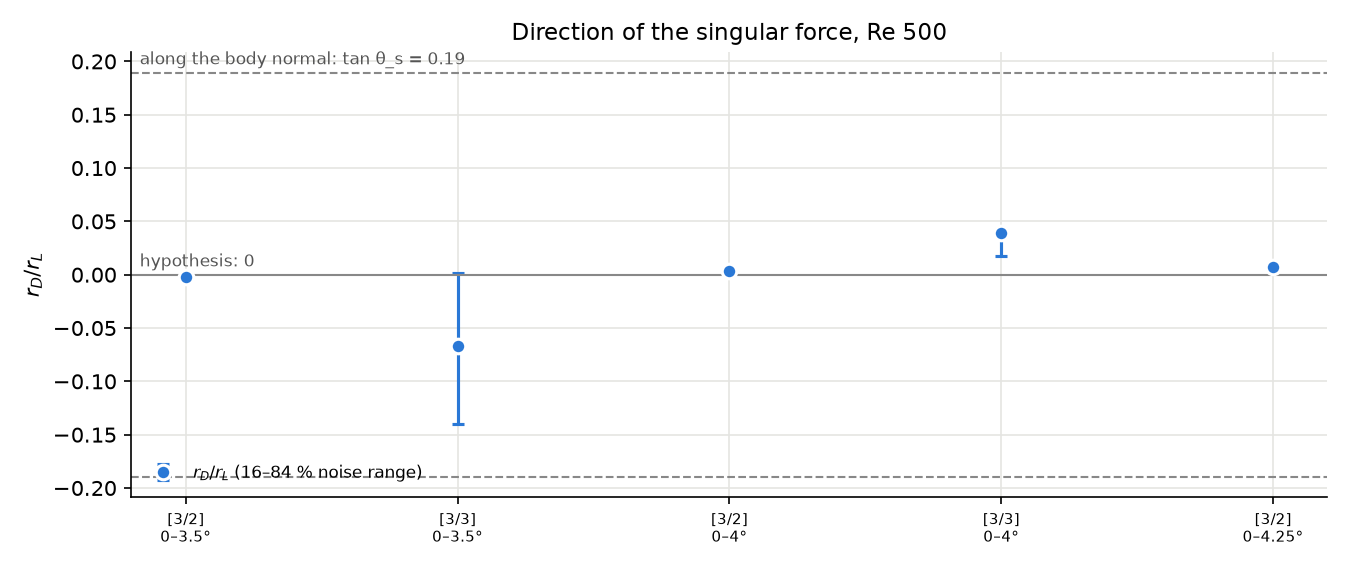
\includegraphics[width=0.85\linewidth]{residue_re500.png}
\caption{$r_D/r_L$ for the shared-denominator fits that reach the noise floor, with $16$--$84\%$ ranges
over 200 noise refits. Lines: the hypothesis (0), and a singular force along the body normal
($\pm\tan\theta_s$).}
\end{figure}

\textbf{Results.}
\begin{itemize}[leftmargin=*]
\item \textbf{[3/2]}, the calibrated order, puts the shared pole at $9.6$--$11.0^\circ$ with
  $r_D/r_L = -0.002$, $+0.003$, $+0.007$ over three windows. $P_D$ itself vanishes at the pole.
\item \textbf{The square-root fit} gives $B_D/(\theta_s B_L) = +0.0049$.
\item Forbidding the pole outright in $\CD$ costs a factor of about $66$ in rms: $\CD$'s singular part is
  small but not zero.
\end{itemize}

\begin{center}\small
\begin{tabular}{p{0.38\linewidth}lp{0.38\linewidth}}
\toprule
verdict rule & outcome & reason\\
\midrule
fixed in advance: all real-pole fits & rejected & driven by low orders that do not fit the data
(rms $10^2$--$10^4\times$ the noise)\\
amended after seeing the data: fits at the noise floor & inconclusive & driven by [3/3], which the
calibration shows cannot discriminate\\
\bottomrule
\end{tabular}
\end{center}

\textbf{Reading.} The calibrated and model-based routes agree on a singular force about $0.3^\circ$ from
the lift axis, as the hypothesis predicts. Neither stated rule confirms it. Its meaning also depends on
Section~\ref{sec:fold}: it describes whatever drives the series' growth, which may not be a real-axis
singularity.

% =====================================================================================
\section{The fold test: first results (Re 500)}\label{sec:fold}

A fold of the steady branch on the real axis would end the branch. It would show up as SIMPLE losing
convergence, $\CL$ steepening like $\sqrt{\alpha_s-\alpha}$, or disagreement (hysteresis) between a chain of
solutions climbing from below and one descending from above. Two chains run on the E800 grid at
production tolerances, which give about $10^{-5}$ precision, ample here.
\begin{itemize}[leftmargin=*]
\item \textbf{Ascending:} $7\to12^\circ$, each angle seeded from the one below, starting from the converged
  $6^\circ$ case.
\item \textbf{Descending:} a cold start at $12^\circ$, then $11\to9^\circ$, each seeded from the one above.
\end{itemize}

\begin{figure}[htbp]\centering
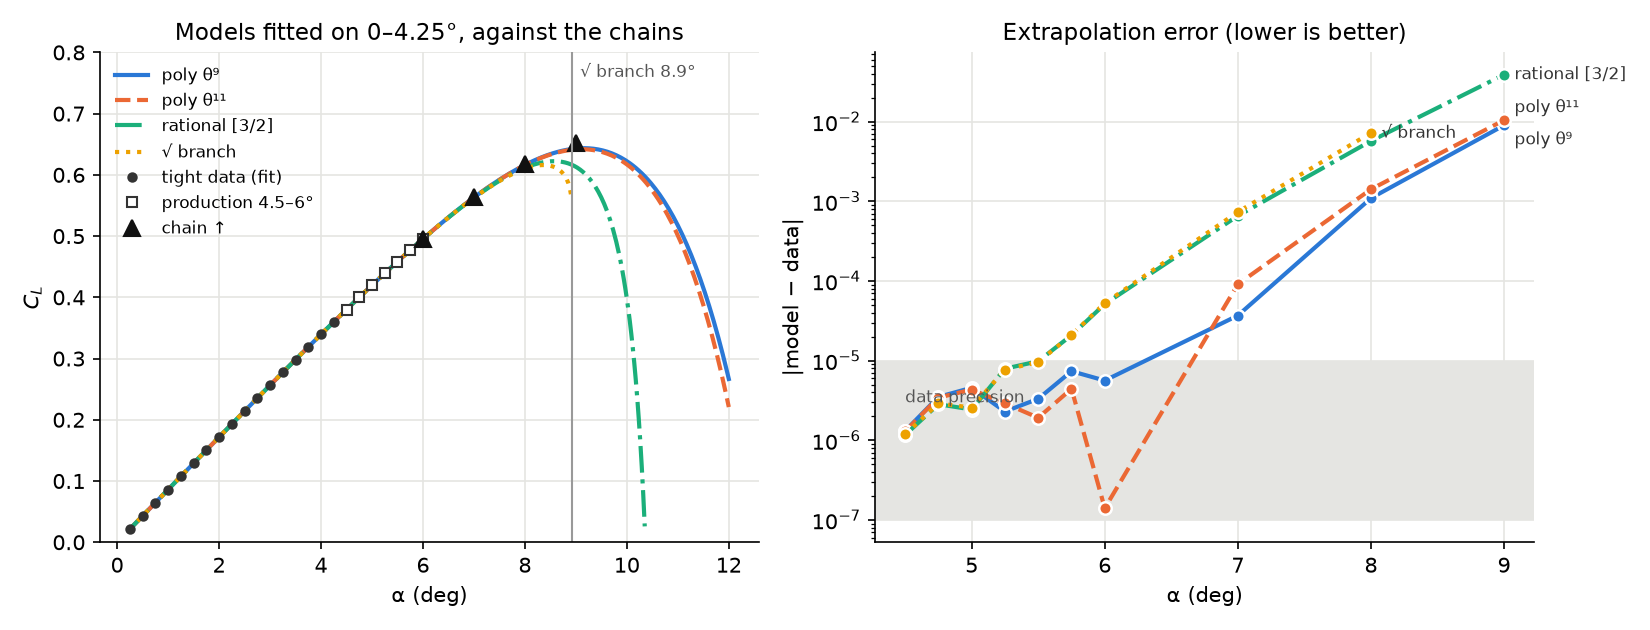
\includegraphics[width=\linewidth]{fold_extrapolation.png}
\caption{Left: models fitted on the tight $0$--$4.25^\circ$ data, against the production data to
$6^\circ$ and the ascending chain. Right: $|\text{model}-\text{data}|$; the grey band is the data
precision.}
\end{figure}

\begin{center}\small
\begin{tabular}{rcccccc}
\toprule
$\alpha$ & $\CL$ (chain) & $\mathrm{d}\CL/\mathrm{d}\alpha$ per degree & poly $\theta^9$ & poly $\theta^{11}$ & Padé [3/2] & $\sqrt{\ }$ branch $8.92^\circ$\\
\midrule
6 & 0.495485 & -- & $+6\times10^{-6}$ & $-1\times10^{-7}$ & $-5\times10^{-5}$ & $-5\times10^{-5}$\\
7 & 0.563141 & 0.068 & $-4\times10^{-5}$ & $-9\times10^{-5}$ & $-7\times10^{-4}$ & $-7\times10^{-4}$\\
8 & 0.617308 & 0.054 & $-1.1\times10^{-3}$ & $-1.4\times10^{-3}$ & $-5.7\times10^{-3}$ & $-7.2\times10^{-3}$\\
9 & 0.652017 & 0.035 & $-9.0\times10^{-3}$ & $-1.0\times10^{-2}$ & $-3.9\times10^{-2}$ & undefined\\
\bottomrule
\end{tabular}\\[2pt]
model minus chain $\CL$; remainders of the chain cases $\le6\times10^{-6}$
\end{center}

\begin{itemize}[leftmargin=*]
\item \textbf{The steady branch continues smoothly through $9^\circ$}, converged to $\le6\times10^{-6}$. Its
  slope \emph{falls} ($0.068 \to 0.054 \to 0.035$ per degree): $\CL$ is approaching a maximum near
  $9$--$9.5^\circ$. A smooth maximum is not a singularity; a fold would make the slope diverge instead.
\item \textbf{The polynomial fits extrapolate 4--10 times better than the singular models,} at every
  angle from $6^\circ$ to $9^\circ$.
\item \textbf{The square-root model's branch point at $8.92^\circ$ is contradicted on this branch.} The
  model has no value past $8.92^\circ$, yet a smooth steady solution exists there. One escape remains: the
  chain may have crossed onto another branch. The descending chain would show that as a disagreement.
\item \textbf{Status:} $9.5$--$12^\circ$ ascending, and the whole descending chain, are still running
  (\path{zero_thickness_plate/progress.py}).
\end{itemize}

% =====================================================================================
\section{Hypothesis register}\label{sec:register}

Origins follow \texttt{HYPOTHESIS\_PROVENANCE.md} in the repository: ``user'' for the user, ``Claude'' for
Claude Code (Claude Opus 5.5), ``ChatGPT'' for suggestions from conversations.

{\small\setlength{\tabcolsep}{4pt}\noindent
\begin{tabularx}{\linewidth}{>{\raggedright\arraybackslash}p{0.25\linewidth}>{\raggedright\arraybackslash}p{0.13\linewidth}>{\raggedright\arraybackslash}X>{\raggedright\arraybackslash}p{0.12\linewidth}}
\toprule
hypothesis & origin & test and evidence & status\\
\midrule
\endhead
The lift is cubic at the origin; $\mathrm{d}\CL/\mathrm{d}\alpha$ is quadratic at small angles & user & deficit
exponent $\to3$; finite, robust $a_3$ for four bodies (Sec.~2, 4) & \supp\\\addlinespace[4pt]
A laminar separation bubble explains the waning cubic dominance & user & bubble analysis
(\path{lsb/HYPOTHESIS_TEST.md}) & \rej\\\addlinespace[4pt]
$a_3$ follows a power law in Re & Claude & local power laws for the airfoils; non-monotonic for both plates
& airfoils only\\\addlinespace[4pt]
The thick plate's non-monotonic $a_3$ comes from its sharp leading edge & Claude & premise false: its
leading-edge radius exceeds NACA0006's & \wdn\\\addlinespace[4pt]
The zero-thickness plate's deficit is non-analytic ($\theta^{3.4}$) & data (H-grid) & orthogonal grid gives
$\theta^{3.10}$ (Sec.~3) & \wdn\\\addlinespace[4pt]
Production data are noise-limited at $10^{-8}$ & Claude & tight re-convergence: a smooth bias of
$10^{-7}$--$10^{-5}$ (Sec.~5) & \rej\\\addlinespace[4pt]
The radius shrinks as $\mathrm{Re}^{-0.63}$; $|a_5|$ grows with Re & Claude (production data) & tight $a_5$:
$-367$, $-376$, $-313$; radius $10.7\to9.4^\circ$ (Sec.~5) & \wdn\ (Re 500--900)\\\addlinespace[4pt]
The singularity is tied to leading-edge bubble formation & Claude & $\CL$'s radius does not track the
bubble angle; $\CA$'s pole does move with Re ($11.5\to7.6^\circ$) & \opn\\\addlinespace[4pt]
Nearest singularity: a real-axis fold near $10.3$--$11^\circ$ & Claude (Padé, AAA, sign pattern) & branch
smooth through $9^\circ$; singular models extrapolate worse than polynomials (Sec.~9) & \weak; decisive runs
pending\\\addlinespace[4pt]
Square-root branch point at $8.92^\circ$ & Claude (model fit) & smooth steady solution at $9^\circ$, falling
slope (Sec.~9) & \rej\ on the ascending branch\\\addlinespace[4pt]
$\CD$ carries the same singularities as $\CL$ & user & $\CD$ shows none consistently; $\CA$, $\CN$ do
(Sec.~7) & partly\\\addlinespace[4pt]
The singular force points along the lift (residue cancellation) & Claude; test design proposed by the
user & calibrated routes: $\approx0.5\%$, $\approx0.3^\circ$; stated rules: rejected / inconclusive
(Sec.~8) & \opn, leaning supported\\\addlinespace[4pt]
The two v14 snapshots differ at the $10^{-9}$ level & Claude, as a precaution & unmeasured; cfd-test upgraded
on 2026-10-20 & \opn\\\addlinespace[4pt]
\bottomrule
\end{tabularx}}

% =====================================================================================
\section{Further tests, in order of priority}\label{sec:next}

\begin{enumerate}[leftmargin=*]
\item \textbf{Finish the fold chains} ($9.5$--$12^\circ$ ascending, $12\to9^\circ$ descending). Check for
  hysteresis at common angles, loss of convergence, and the location of the $\CL$ maximum. Re-converge
  the cases around the maximum at tight tolerance.
\item \textbf{If there is no fold, find where the singularity is.}
  \begin{itemize}
  \item Refit Padé/AAA including the chain data ($6$--$12^\circ$, precision $10^{-5}$), to see whether the
    pole leaves the real axis as a complex pair.
  \item Compute the leading eigenvalues of the linearised steady problem along the branch. A fold needs a
    real eigenvalue crossing zero; the marginal-stability tools of the NACA0012 campaign
    (\texttt{run\_marginal.sh}) apply.
  \item Locate the shedding onset (Hopf) of the zero-thickness plate at Re 500. It does not end the
    steady branch, but it decides whether the steady loads beyond it are physically relevant to the
    step response.
  \end{itemize}
\item \textbf{Complete the tight data.}
  \begin{itemize}
  \item The 12 angles above about $3^\circ$ that are not converged (Re 500: $4.5$--$5^\circ$; Re 700:
    $4$--$4.5^\circ$; Re 900: $0.75$, $3$--$4.5^\circ$).
  \item The Re 900 $0^\circ$ case.
  \item Re 200--400, 600 and 800, to rebuild $a_5(\mathrm{Re})$, the radius against Re, and the drag
    coefficients against Re.
  \end{itemize}
\item \textbf{Re-converge the other three bodies,} to verify their $a_5$, $a_7$ and $d_4$.
\item \textbf{Mesh sensitivity} of $a_5$ and of $d_0$--$d_4$ (E560 against E800, at tight tolerance).
\item \textbf{Measure the build gap:} continue one converged Re 700 case for a few hundred tight iterations
  on the upgraded cfd-test.
\item \textbf{Residue test at Re 700 and 900} once their singular feature is robust, and $\CA$ against $\CN$
  residues at a shared pole.
\item \textbf{Theory for the drag scales:} compare the excess of $d_0$ over Blasius, and $\eta(\mathrm{Re})$,
  with second-order boundary-layer and trailing-edge (triple-deck) corrections.
\item \textbf{Then the programme's goal:} step responses against these steady baselines.
\end{enumerate}

% =====================================================================================
\appendix
\section{Reproducibility}

Scripts are run with the \texttt{research} conda environment from \texttt{static\_airfoil/}. All code and
notes are in the repository \url{https://github.com/Imdadullah-Raji/viscous_wagner}; force histories and
fields stay in the working tree.

\begin{center}\small
\resizebox{\linewidth}{!}{%
\begin{tabular}{ll}
\toprule
analysis & script (outputs in a folder of the same name)\\
\midrule
stress test, four bodies, production & \texttt{analysis/cubic\_stress\_test.py}\\
tight against production, odd Legendre fits & \texttt{analysis/tight\_compare.py 500 700 900 --drop}\\
Padé (routes A, B) and AAA (route C) & \texttt{analysis/pade\_singularity.py 500 [--prod]}\\
drag, body axes, singularities by component & \texttt{analysis/drag\_even\_fit.py 500 700 900 [--prod|--bodies]}\\
residue test & \texttt{analysis/residue\_test.py 500}\\
fold test & \texttt{analysis/fold\_check.py}\\
re-convergence drivers & \texttt{zero\_thickness\_plate/tighten\_case.sh}, \texttt{tight/}\\
fold chains, progress bars & \texttt{zero\_thickness\_plate/fold/fold\_chain.sh}, \texttt{progress.py}\\
\bottomrule
\end{tabular}}
\end{center}

The running record, with every number above and the reasoning behind each step, is
\path{analysis/CUBIC_STRESS_TEST.md}, sections 1--11.

\end{document}
